%!TEX root=../document.tex

\section{Einführung}
Dieses Protokoll-Template soll helfen den Laborübungsteil entsprechend dokumentieren zu können. Diese Vorlage ist in \LaTeX  verfasst.

\subsection{Ziele}
Hier werden die zu erwerbenden Kompetenzen und deren Deskriptoren beschrieben. Diese werden von den unterweisenden Lehrkräften vorgestellt.

Dies kann natürlich auch durch eine Aufzählung erfolgen:

\begin{itemize}
	\item \textbf{Lorem ipsum:} dolor sit amet, consetetur sadipscing elitr
	\item sed diam nonumy eirmod tempor invidunt ut labore et dolore magna aliquyam erat
	\item ut labore et dolore magna aliquyam erat, sed diam voluptua
\end{itemize}


\subsection{Voraussetzungen}
Welche Informationen sind notwendig um die Laborübung reibungslos durchführen zu können? Hier werden alle Requirements der Lehrkraft detailliert beschrieben und mit Quellen untermauert.

Hier zum Beispiel die Architektur der \textit{Common Object-Request-Broker Architecture}:
\begin{figure}[!h]
	\begin{center}
		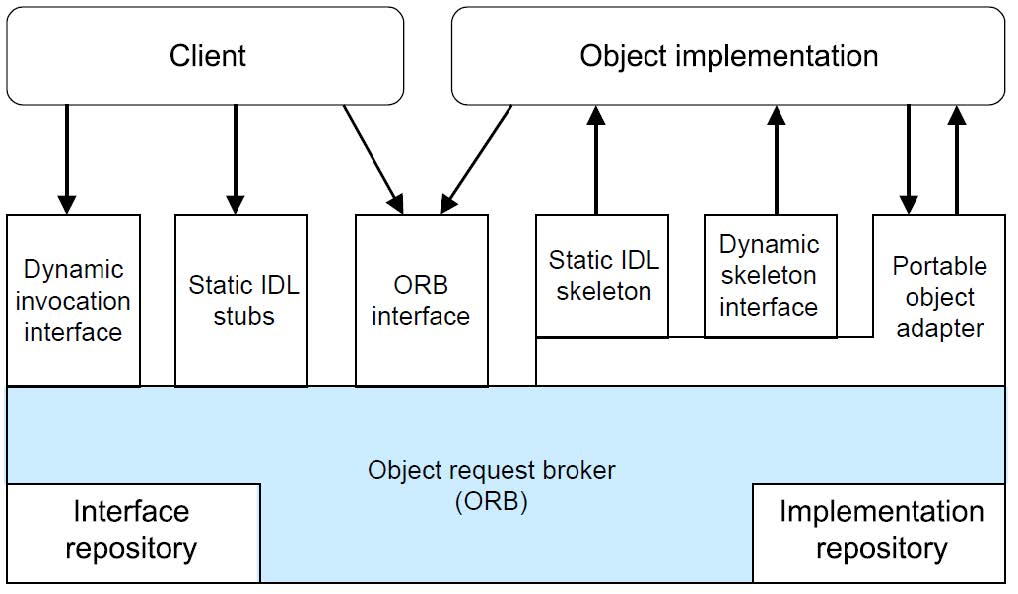
\includegraphics[width=0.5\linewidth]{images/corba.jpg}
		\caption{Common Object-Request-Broker Architecture \cite{tanenbaum2007verteilte}}
		\label{broker}
	\end{center}
\end{figure}


\subsection{Aufgabenstellung}
Hier wird dann die konkrete Aufgabenstellung der Laborübung definiert.

Nun kommt ein Seitenumbruch, um eine klare Trennung der Schülerarbeit zu bestimmen.
\clearpage
